% Paper, encoding and fonts settings
\documentclass[a4paper]{report}
\usepackage{geometry}
\usepackage[utf8]{inputenc}
\usepackage[T1]{fontenc}
\usepackage{polski}
\usepackage{indentfirst}
\usepackage[polish]{babel}

% Graphics
\usepackage{graphicx}
\graphicspath{{./graphics/}}

% Math, physics and numbers
\usepackage{amsmath}
\usepackage{siunitx}
% Proper decimal separation
\usepackage{icomma}

% Extra features and enhancements
\usepackage{cite}
% Tables
\usepackage{booktabs}
\usepackage{multirow}
% Listings
\usepackage{minted}
% Make sure that hyperref is last loaded package
\usepackage[hidelinks]{hyperref}

% Renew some commands to ensure Polish names
\renewcommand\listoflistingscaption{Spis listingów}
% There is no Polish locale for units, French is the closest one
\sisetup{locale = FR}

\author{Wojciech Ptasiński \and Maciej Ziaja}
\title{Raport z~projektu indywidualnej organizacji studiów}

\begin{document}

\maketitle

% Introductory pages
\begin{abstract}
Abstract
\end{abstract}

\tableofcontents

% Sections
\section{Wstęp}
Przedmiotem projektu jest konstrukcja zestawu wybranych algorytmów robotyki dla
mobilnych pojazdów autonomicznych oraz ich symulacja w środowisku ROS (Robotics
Operating
System). Platforma ROS pozwala na szybkie prototypowanie oprogramowania robotów
w wirtualnych środowiskach symulacyjnych z~wykorzystaniem systemu operacyjnego
Linux.
Modelowanie obiektów i~konstrukcja algorytmów w językach programowania Python
oraz C++ z użyciem systemu ROS daje możliwość łatwego przenoszenia
oprogramowania na systemy wbudowane.

Wybrane algorytmy obejmują tematy predykcji położenia, przetwarzania danych
wizyjnych, wykrywania elementów otoczenia oraz planowania toru jazdy. Wyniki
projektu mogą być podstawą do konstrukcji platformy sprzętowej realizującej
algorytmy. Gotowa platforma może stanowić podstawę do dalszych prac nad
wykorzystaniem sztucznej inteligencji i~algorytmów sterowania w~systemach
mobilnych.

Dodatkowo, w~ramach projektu, zrealizowano analizę biznesową produkcji robotów
autonomicznych w~lokalnych warunkach, na podstawie danych o istniejących
firmach działających w~rozpatrywanej dziedzinie.

Środowisko ROS znajduje zastosowania w przemyśle oraz jest narzędziem
wykorzystywanym przy pracach nad dynamicznie rozwijającą się technologią
pojazdów autonomicznych.

\chapter{Organizacja}


\section{Podział zadań}
Podział zadań między studentów przedstawiono w~tabeli \ref{tab:org}.
Ilość zadań przydzielonych zadań oraz ich charakter odpowiada efektom
kształcenia realizowanym przez studentów.

\begin{table}[h]
\begin{tabular}{ll}
\toprule
\multicolumn{1}{c}{Wojciech Ptasiński}   & \multicolumn{1}{c}{Maciej Ziaja} \\
\midrule
Konfiguracja środkowiska ROS             & Przygotowanie skryptów
                                           konfiguracyjnych \\
Przygotowanie modelu robota i symulatora & Implementacja sterowników czujników
                                           IMU \\
Opracowanie odometrii robota             & Implementacja filtru Kalmana \\
Implementacja sterowania robotem         & Opracowanie i implementacja systemu
                                           AHRS \\
Analiza biznesowa                        & Opracowanie prototypu systemu
                                           wizyjnego \\
                                         & Przygotowanie prototypu sprzętowego
                                           mikroprocesora \\
                                         & Analiza biznesowa \\
\bottomrule
\end{tabular}
\caption{Tabela podziału zadań między studentów realizujących projekt}
\label{tab:org}
\end{table}

\section{Środowisko prototypowania robotów ROS}
Robot Operating System (ROS) to framework do pisania oprogramowania robotów.
Jest to zbiór narzędzi, bibliotek i~konwencji, które mają na celu uproszczenie
zadania tworzenia złożonych zachowań robotów na wielu różnych platformach
robotyki.

Architektura środowiska uruchomieniowego ROS to sieć procesów
\textit{peer-to-peer} (potencjalnie rozproszona na komputerach), które są luźno
połączone za pomocą infrastruktury komunikacyjnej ROS.

\textbf{Peer-to-peer (P2P)} to model komunikacji, w~którym każda ze stron ma te
same uprawnienia i każda ze stron może zainicjować sesję komunikacyjną.
ROS implementuje kilka różnych stylów komunikacji, w~tym synchroniczną
komunikację w stylu RPC za pośrednictwem usług, asynchroniczne przesyłanie
danych do tematów i przechowywanie danych na serwerze parametrów.

\textbf{RPC (ang. \textit{remote procedure call})} polega na tym ,że gdy
program komputerowy powoduje wykonanie procedury (podprogramu), w~innej
przestrzeni adresowej (zwykle na innym komputerze w sieci współdzielonej),
która jest kodowana tak, jakby była normalnym (lokalnym) wywołaniem procedury,
bez programisty jawnie kodującego szczegóły dotyczące zdalnej interakcji.

\section{Komunikacja publish-subscribe}
W architekturze oprogramowania na platformie ROS, komunikacja odbywa się
zgodnie protokołem przesyłania wiadomości \textbf{publish-subscribe} (rys.
\ref{fig:pubsub}), realizujące połączenie pomiędzy poszczególnymi
\textbf{węzłami}.
Protokół publish-subscribe, polega na tym, że węzły wysyłające wiadomości,
nazywane \textbf{węzłami publikującymi}, nie określają
do jakiego konkretnego odbiorcy, nazywanego \textbf{węzłem subskrybującym}, ma
dana wiadomość trafić.
W zamian, kategoryzują wysyłane wiadomości na klasy, które z~kolei nazywamy
\textbf{tematami}, bez żadnej informacji do jakiego,
jeżeli do jakiegokolwiek węzła, ma ona trafić.
Cała komunikacja odbywa się dzięki serwerowi (nazywanemu \textbf{ROS Master}),
który umożliwia węzłowi subskrybującemu zidentyfikowanie źródła danych będących
przedmiotem zainteresowania.
Ten paradygmat daje możliwość istnienia wielu jednoczesnych
węzłów publikujących i~subskrybujących.
Jeden węzeł publikujący może publikować dane do wielu węzłów subskrybujących
lub zasubskrybować się u jednego z innych wydawców w~bieżącym systemie.

\begin{figure}
  \centering
  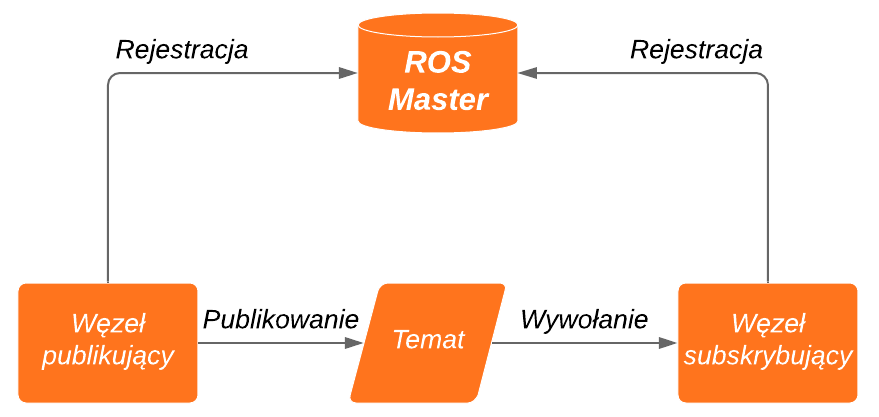
\includegraphics[width=105mm]{graphics/ROSflow.png}
\caption{Schemat przepływowy danych w protokole publish-subscribe, na
platformie ROS}
  \label{fig:pubsub}
\end{figure}

W~ROS węzeł jest jednostką lub procesem, który wykonuje pewną formę obliczeń
i/lub przetwarzania i akwizycji sygnałów.
Urządzenia i~systemy wykorzystywane przez pojazd, który jest omawiany
w~niniejszym projekcie, można przedstawić za pomocą węzłów.
Na przykład, węzeł na dane enkodera, węzeł dla urządzenia LiDAR,
węzeł do autonomicznej jazdy (w tym nawigacja, planowanie trasy, unikanie
przeszkód), węzeł do wizualizacji.
Węzły porozumiewają się ze sobą za pomocą struktur danych (określane jako typy
wiadomości) które składają się z~wymaganych pól będących typu liczba całkowita,
liczba zmiennoprzecinkowa, wartość logiczna czy też obiekt pewnej klasy.
Jeśli węzeł chce się komunikować z~innym węzłem, opublikuje wiadomość
o~określonej strukturze do tematu, a~inny węzeł zasubskrybuje ten temat
(oczekując określonego typu wiadomości i~pola) i~gromadząc wymagane dane.
Przy każdej dostarczonej wiadomości, w~węźle subskrybującym aktywowane jest
wywołanie (ang. \textit{callback}), w~którym zdefiniowane są, dalsze czynności
powiązane z~tą wiadomością np. przetworzenie w określony sposób i~przekazanie
do kolejnego węzła.

\section{Model URDF}
\textbf{Unified Robot Description Format (URDF)} to specyfikacja XML opisująca
robota. Roboty formacie URDF są reprezentowane w strukturze drzewa, które
przedstawia stworzoną hierarchię połączeń pomiędzy poszczególnymi członami
modelu. Specyfikacja zakłada, że robot składa się ze sztywnych elementów
połączonych ze sobą. Specyfikacja obejmuje kinematyczny i dynamiczny opis,
wizualną reprezentację oraz model zderzeniowy robota.

Na poziomie implementacji plik URDF jest po prostu plikiem tekstowym
zawierającym znaczniki XML: określone słowa kluczowe, które ROS rozpoznaje jako
część URDF.

Niektóre ze znaczników XML odnoszą się do innych plików lub modeli 3D części
robotów, co pozwala korzystać z plików zewnętrznych w celu szybkiego włączenia
szczegółowego kształtu wraz z kolorystyką.

Opis robota składa się z zestawu członów(ang. \textit{links}) i~zestawu
elementów łączących ze sobą człony(\textit{ang. joints}).

\begin{figure}[h]
\centering
\subfloat[Złącze
(\textit{joint})]{{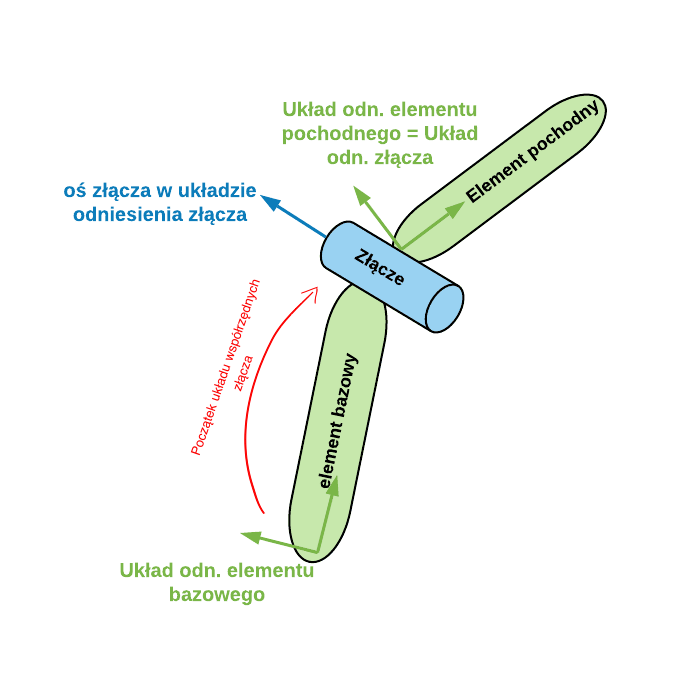
\includegraphics[width=7cm]{graphics/joint2.png} }}%
\qquad
\subfloat[Człon robota
(\textit{link})]{{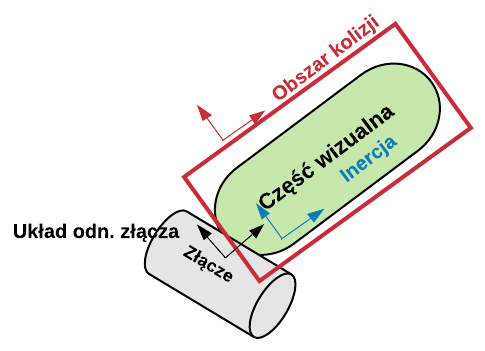
\includegraphics[width=7cm]{graphics/link.png} }}%
\caption{Elementy struktury opisu robota w formacie URDF.}%
\label{fig:linkjoint}
\end{figure}

\textbf{Człon robota} (\textit{link}) opisuje sztywny korpus o bezwładności,
cechach wizualnych i właściwościach kolizji.

\textbf{Złącze}(\textit{joint}) opisuje kinematykę i dynamikę złącza,
umiejscowienie połączenia, element bazowy oraz element pochodny, między którymi
stworzone jest dane złącze.

\section{Środowisko symulacyjne}
Symulacja robota pomaga obniżyć całkowity koszt integracji. Dzieje się tak
głównie dzięki możliwości symulowania aplikacji w świecie rzeczywistym bez
fizycznych kosztów związanych z tym faktem. Symulacja robota również zmniejsza,
a często nawet eliminuje potrzebę wprowadzania zmian w systemie po jego
zainstalowaniu, ponieważ już udowodniono, że jego procesy działają.

Spośród dostępnych otwarto-źródłowych symulatorów 3D, w celu zasymulowania 
pracy robota oraz pomiarów ze skanera LIDAR, wybrano symulator \textit{Gazebo}.
Głównym powodem tego wyboru jest kompatybilność z wykorzystywaną platformą ROS.
Oprócz tego, Gazebo zapewnia wysokowydajne silniki fizyki, realistyczne
renderowanie środowisk, w tym wysokiej jakości oświetlenie, cienie i tekstury.

\begin{figure}
  \centering
  
\includegraphics[width=40mm]{graphics/gazebologo.png}
  \caption{Logo symulatora Gazebo 3D}
  \label{fig:gazebologo}
\end{figure}

Istotną cechą tego symulatora jest możliwość generowania danych czujników,
opcjonalnie z szumem, ze skanerów laserowych, kamer 2D/3D, czujników w~stylu
Kinect, czujników kontaktowych, siły momentu obrotowego i innych.

Obslugiwany przez symulator ROS format SDF opisuje obiekty i~środowisko dla
symulacji, wizualizacji i~sterowania robotem.
Pozwala dokładnie opisać
wszystkie aspekty robota, a~w~razie potrzeby, w~łatwy sposób można go
przekonwertować na format URDF.
Oprócz możliwości tworzenia własnych robotów Gazebo zapewnia kilka modeli,
gotowych do przetestowania.

\section{Symulacja omni robota}
Na poniższym obrazku znajduje się wizualizacja omni robota, który został
stworzony dla celów realizacji projektu.
Początkowo poszczególne części
zostały zaprojektowane jako siatka graficzna, wykorzystując do tego specjalne
programy graficzne, a~następnie wszystkie stworzone elementy robota zostały
zintegrowane ze sobą w formacie URDF.

Wykorzystując wspomniany format (URDF), stworzono odpowiedni model, który
opisuje również momenty bezwładności poszczególnych elementów, co pozwala na
odwzorowanie tego, jak zachowałby się podobny robot w świecie rzeczywistym.

Na robocie znajduje się platforma, na której w dalszym etapie tworzenia modelu,
został zamontowany skaner laserowy LiDAR.

\begin{figure}
  \centering
  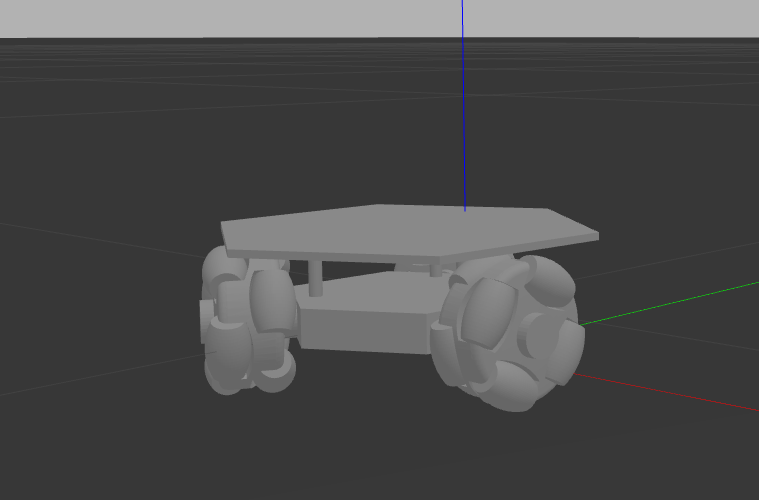
\includegraphics[width=140mm]{graphics/robot.png}
  \caption{Symulacja omni-robota}
  \label{fig:forklift}
\end{figure}
\newpage


\section{Filtr Kalmana i system AHRS}
System AHRS (ang. \textit{attitude and heading reference system}) pozwala na
wyznaczenie orientacji obiektu w~przestrzeni.
Systemu tego typu znajdują szerokie zastosowanie w~pojazdach autonomicznych.

System AHRS można podzielić na dwie główne części: system czujników oraz system
predykcji orientacji w~przestrzeni.
Fragment systemu odpowiedzialny za działanie czujników stawia wyzwania związane
z~obsługą sprzętu oraz jego kalibracją.
Algorytm predykcji pozwala na fuzję danych z~zespołu czujników w~celu
określenia orientacji obiektu w~przestrzeni.

Wynikiem działania systemu AHRS jest wektor trzech wartości reprezentujących
obrót obiektu wokół osi trójwymiarowego układu współrzędnych.
Kąty obrotu noszą nazwę \textit{kątów Eulera}, ich ideowym odpowiednikiem
w~terminologii lotniczej są kąty \textit{roll, pitch, yaw}.

\subsection{Czujniki systemu AHRS i implementacja sprzętowa}
W~celu określenia orientacji obiektu w~przestrzeni konieczny jest zestaw
czujników.
Do wyznaczenia pełnej orientacji w~przestrzeni trójwymiarowej stosuje się
zazwyczaj zestaw: akcelerometru, żyroskopu oraz magnetometru.
Akcelerometr i~żyroskop tworzą razem zestaw nazywany IMU (ang \textit{inertial
measurement unit}).
System IMU pozwala na wyznaczenie kątów odchylenia obiektu od pionu
(\textit{roll} oraz \textit{pitch}), co w~wielu zastosowaniach jest
wystarczające.
Aby uzyskać pełne współrzędne orientacji obiektu w~przestrzeni należy użyć
także magnetometru, który pozwala określić kąt obrotu wokół osi pionowej
(\textit{yaw}).

W~projekcie użyto układu \textit{MinIMU-9 v5} firmy \textit{Pololu}
o~dziewięciu stopniach swobody (trzy stopnie swobody na każdy z~czujników).
\textit{MinIMU} zawiera zestaw: układ IMU \textit{LSM6DS33} oraz magnetometr
\textit{LIS3MDL}.
Komunikacja z czujnikami odbywa się poprzez magistralę \textit{I2C}, przy czym
każdy z trzech czujników ma osobny adres i~wymaga oddzielnej obsługi
komunikacji.
Czujniki wchodzące w skład systemu AHRS wymagają kalibracji, co jest
szczególnie ważne przypadku magnetometru.

\subsubsection{Żyroskop}
Żyroskop to przyrząd pozwalający określić prędkość obiektu kątową w~trzech
osiach.
W~spoczynku żyroskop powinien dawać zerowe odczyty ze wszystkich osi.
Jest to podstawowy czujnik pozwalający określić orientację obiektu
w~przestrzeni.
Wyznaczenie kątów obrotu wymaga jedynie całkowania odczytu z~żyroskopu
(ponieważ prędkość kątowa to pochodna kąta obrotu).
Niestety sam żyroskop nie jest wystarczający aby precyzyjnie orientować obiekt
w~przestrzeni, ze względu na zjawisko dryftu (ang. \textit{gyroscope drift}).
Żyroskop jest mało podatny na szumy pomiarowe o~małej częstotliwości, natomiast
jest wrażliwy na pojawianie się stałych, ale niewielkich błędów w~odczytach.
Ze względu na konieczność całkowania danych z~żyroskopu te małe błędy są
kumulowane, w~wyniku czego wraz z~upływem czasu, orientacja na podstawie
działania żyroskopu staje się coraz mniej wiarygodna.
Dlatego w celu precyzyjnego ustalania orientacji w~przestrzeni konieczne jest
użycie żyroskopu w~parze z akcelerometrem oraz zastosowanie algorytmu fuzji
danych.

\subsubsection{Akcelerometr}
Akcelerometr to czujnik pozwalający mierzyć przyspieszenie kątowe obiektu.
W stanie spoczynku osie poziomie akcelerometru powinny wskazywać zerowe
odczyty, natomiast oś pionowa powinna wskazywać wartość przyspieszenia
ziemskiego.

Akcelerometr jest wolny od zjawiska dryftu, natomiast jest wrażliwy na szumy
pomiarowe o~dużych częstotliwościach.
Przeciwna natura niedokładności akcelerometru oraz żyroskopu sprawia, że
najlepiej pracują one w parze, z~użyciem algorytmu fuzji danych.

W~czujnikach IMU często dokonuje się kalibracji błędu zera (addytywnego).
Należy wykonać to w trakcie spoczynku systemu na płaskiej powierzchni.
Oś pionowa akcelerometru nie powinna być kalibrowana.

\subsubsection{Magnetometr}
Magnetometr mierzy indukcję pola magnetycznego w~trzech kierunkach.
Ponieważ między biegunami Ziemi przebiegają linie pola magnetycznego, to
magnetometr może być użyty do wyznaczenia orientacji obiektu w przestrzeni
(jako kompas).
Oś magnetometru leżąca w kierunku północ-południe wskazuje wartości maksymalne
indukcji, osie prostopadłe wskazują wartości minimalne.

Kluczowym zagadnieniem jest kalibracja magnetometru, który jest obciążony
zarówno błędem addytywnym (nazywanym z ang. \textit{hard iron}), jak
i~multiplikatywnym (nazywanym z ang. \textit{soft iron}).
Odczyty magnetometru są wrażliwe na zakłócenia powstałe w wyniku działań innych
części układów robotyki.
Z~tego powodu kalibracja magnetometru jest koniecznością, magnetometr
nieskalibrowany jest obciążony błędami uniemożliwiającymi poprawne działanie
systemu AHRS.

\subsection{Kalibracja czujników}
W przypadku czujników IMU kalibracja polega na uśrednieniu odczytu $ n $
wartości w~trakcie spoczynku na równym podłożu.
Kolejne odczyty należy korygować o~zapisaną wartość średniej.

W przypadku magnetometru w czasie kalibracji należy nim poruszać, tak aby
każda oś jego pomiaru obróciła się w~przestrzeni o~kąt pełny.
W~przypadku poprawnie skalibrowanego magnetometru pomiary o~maksymalnych
wartościach powinny mieć na wykresie kształt okręgu ze środkiem w~początku
układu współrzędnych.
W przypadku wystąpienia błędu \textit{hard iron} środek okręgu jest
przesunięty, natomiast w~wyniku działania błędu \textit{soft iron} następuje
zniekształcenie okręgu.

Ważne jest aby kalibracji dokonać w~odpowiedniej kolejności, najpierw należy
wyznaczyć \textit{hard iron}, a~potem \textit{soft iron}.
Obliczenie błędu multiplikatywnego wymaga, aby błąd addytywny był już
zniwelowany.
Błąd \textit{hard iron} jest średnią ze skrajnych wartości $ n $ pomiarów, co
przedstawiono na wzorze \ref{eq:hard_iron}, gdzie $ \vec{m_n} $ to wektor
pomiarów z~czujnika.
\begin{equation}
	\vec{e_{hard}} = 
		\frac{max\left(\vec{m_n}\right) + min\left(\vec{m_n}\right)}{2}
\label{eq:hard_iron}
\end{equation}
Błąd \textit{soft iron} należy wyznaczyć według wzorów od
\ref{eq:hard_iron_beg} do \ref{eq:hard_iron_end}.
\begin{gather}
	\vec{r} =
		\frac{max\left(\vec{m_n}\right) - min\left(\vec{m_n}\right)}{2}
	\quad
	\vec{r} = \left[r_x, r_y, r_z\right] \\
\label{eq:hard_iron_beg}
	r_a = \frac{r_x + r_y + r_z}{3} \\
	\vec{e_{soft}} =
		\left[ \frac{r_a}{r_x}, \frac{r_a}{r_y}, \frac{r_a}{r_z}\right]
\label{eq:hard_iron_end}
\end{gather}
Ostatecznie odczyty magnetometru należy korygować według wzoru
\begin{equation}
	\vec{m_{fixed}} = \left(\vec{m} - \vec{e_{hard}}\right) \cdot \vec{e_{soft}}
\end{equation}

\subsection{Implementacja obsługi czujników w systemie operacyjnym Linux}
Obsługę czujników zdecydowano się oprzeć na systemie Linux, który jest również
bazą dla środowiska ROS.
Jądro systemu Linux udostępnia dostęp do magistrali komunikacji \textit{I2C}
poprzez wywołania systemowe (ang. \textit{system calls}).
Urządzenia peryferyjne w~systemach pochodnych systemu \textit{UNIX} są
reprezentowane przez pliki znakowe.
W~celu nawiązania połączenia z~czujnikiem należy otworzyć plik urządzenia
znakowego \textit{I2C} za pomocą wywołania \mintinline{c}{open()}.
Pliki urządzeń peryferyjnych znajdują się w~katalogu \texttt{/dev/}.
Połączenie nawiązuje się wywołaniem
\mintinline{C}{ioctl(device_handle, I2C_SLAVE, i2c_address);}, gdzie
\mintinline{C}{device_handle} to deskryptor otwartego pliku urządzenia
znakowego, \mintinline{C}{I2C_SLAVE} to stała określająca tryb działania
urządzania, a \mintinline{C}{i2c_address} to adres urządzenia podłączonego do
magistrali \textit{I2C}.
Wymiana z~urządzeniami odbywa się poprzez zapis i~odczyt danych z pliku
urządzenia, za pomocą wywołań \mintinline{C}{read()} oraz
\mintinline{C}{write}.
Istotne jest aby odczytywać i~zapisywać odpowiednią liczbę bajtów, oraz
poprawnie skalować odczyty.
Informacje na temat formatu przesyłanych danych znajdują się w~notach
katalogowych czujników.
Istnieją dodatkowe biblioteki ułatwiające pracę z~urządzeniami \textit{I2C}
(np. \textit{SMBUS}), jednak opisany sposób jest najbardziej uniwersalny.
Utworzona biblioteka komunikacji z~czujnikami \textit{MinIMU-9 v5} będzie
działała na każdym urządzeniu z~systemem Linux, którego jądro obsługuje
komunikację \textit{I2C}.

Program napisano w~języku C\texttt{++} odpowiednio opakowując kod języka C.
Błędy zgłaszane przez system \textit{errno} obsłużono przez wyjątki.
Adresy rejestrów i~urządzeń \textit{I2C} zapisano w~silnie typowanych
wyrażeniach wyliczeniowych, które parametryzują szablony klas urządzeń
magistrali \textit{I2C}.
Oprogramowanie obsługi czujników udostępniono w~postaci statycznie łączonej
biblioteki programistycznej.

\subsection{Filtr Kalmana}
Filtr Kalma jest algorytmem estymacji stanu modelu dynamicznego.
Algorytmy tego typu określają wewnętrzny stan obiektu na podstawie pomiarów
wejścia i~wyjścia tego układu.
Filtr wykonuje estymacje rekurencyjnie, na podstawie wcześniejszych obliczeń,
a~szacunki są optymalne, zakładając że błędy pomiarowe mają rozkład
normalny oraz układ jest liniowy.
Jeżeli układ dyskretny opisany jest równaniami
\ref{eq:state_kalman}~i~\ref{eq:meas_kalman}, gdzie:
\begin{description}
	\item[$x\left(t\right)$] to wektor stanu w~funkcji czasu,
	\item[$y\left(t\right)$] to wektor wyjścia układu (pomiaru) w~funkcji czasu,
	\item[$A$] to macierz systemowa (przejścia),
	\item[$B$] to macierz wejścia,
	\item[$H$] to macierz wyjścia (pomiaru),
	\item[$v\left(t\right), u\left(t\right)$] to wektory szumu, kolejno
		procesu oraz pomiaru.	
\end{description}
\begin{align}
x\left(t + 1\right) &= Ax\left(t\right) + Bu\left(t\right) + v\left(t\right)
\label{eq:state_kalman} \\
y\left(t\right) &= Hx\left(t\right) + w\left(t\right)
\label{eq:meas_kalman}
\end{align}

Działanie filtru Kalmana składa się z~dwóch faz: fazy predykcji (\textit{a
priori}) oraz aktualizacji (\textit{a posteriori}).
Faza predykcji (ekstrapolacji) polega na wyznaczeniu stanu układu w~nowej
chwili czasu na podstawie modelu układu oraz wcześniejszego stanu.
W~czasie predykcji wyznaczana jest również nowa macierz niepewności
(kowariancji estymacji).
Predykcja odbywa się według wzorów
\ref{eq:predict_state}~i~\ref{eq:predict_unc}, gdzie:
\begin{description}
	\item[$\hat{x}_a\left(t\right)$] to estymacja \textit{a priori} wektora stanu
	w~funkcji czasu,
	\item[$\hat{x}_p\left(t\right)$] to estymacja \textit{a posteriori} wektora
	stanu w~funkcji czasu,
	\item[$P_a\left(t\right)$] to macierz kowariancji estymacji stanu \textit{a
	priori} w~funkcji czasu,
	\item[$Q$] to macierz kowariancji szumu procesu.
\end{description}
\begin{align}
	\hat{x}_a\left(t\right) &= A\hat{x}_p\left(t-1\right) + Bu\left(t-1\right)
	\label{eq:predict_state} \\
	P_a\left(t\right) &= AP_p\left(t-1\right)A^T + Q
	\label{eq:predict_unc}
\end{align}
Kolejnym etapem jest aktualizacja, która odbywa się na podstawie pomiaru
wyjścia układu.
Ma ona za zadanie poprawić estymację stanu, uwzględniając różnicę między
rzeczywistym pomiarem wyjścia, a~jego wartością obliczoną \textit{a priori}
przy pomocy stanu z~fazy predykcji.
Kluczowym elementem filtru Kalmana jest \textit{wzmocnienie Kalmana}, które
reprezentuje balans ufności w~predykcję \textit{a priori} (według modelu) oraz
w~pomiary wyjścia \textit{a posteriori}.
W~trakcie fazy aktualizacji, wyznaczane jest także nowe
\textit{wzmocnienie Kalmana}.
Intuicyjnie można powiedzieć, że wzmocnienie jest wyznaczane tak, by najlepiej
balansować pomiędzy przewidywaniem stanu według modelu matematycznego
(niedoskonałego, a~także nie obejmującego zakłóceń procesu) oraz przewidywaniem
według pomiaru (obarczonego szumem pomiarowym).
Faza aktualizacji odbywa się zgodnie ze wzorami od \ref{eq:kalman_update_K} do
\ref{eq:kalman_update_P}, gdzie:
\begin{description}
	\item[$K\left(t\right)$] to \textit{wzmocnienie Kalmana} w~funkcji czasu,
	\item[$\hat{P}_p\left(t\right)$] to macierz kowariancji estymacji stanu
	\textit{a posteriori} w~funkcji czasu,
	\item[$R$] to macierz kowariancji szumu pomiarowego.
\end{description}
\begin{gather}
	K\left(t\right) = P\left(t\right) H^T \cdot
	\left(HP_a\left(t\right)H^T + R\right)^{-1}
\label{eq:kalman_update_K} \\
	\hat{x}_p\left(t\right) = \hat{x}_a\left(t\right) +
	K\cdot\left(y\left(t\right) - H \hat{x}_a\left(t\right)\right)
\label{eq:kalman_update_x} \\
	P_p\left(t\right) = \left(I - K\left(t\right)H\right) \cdot P_a\left(t\right)
	\label{eq:kalman_update_P}
\end{gather}

\subsection{Zastosowanie filtru Kalmana w~fuzji danych pochodzących z~czujnika
            IMU}
Filtr Kalmana można zastosować, aby oszacować orientację obiektu w~przestrzeni
na podstawie odczytów z~czujnika IMU.
Fuzja danych przy pomocy filtru pozwala zniwelować niedoskonałości żyroskopu
(dryft) oraz akcelerometru (szumy pomiarowe).
Zazwyczaj dane z~żyroskopu są używane w roli wejścia systemu, na etapie
predykcji, a~pomiary z~akcelerometru są wykorzystywane podczas fazy
aktualizacji.
Czujniki IMU pozwalają jedynie na określenie kątów \textit{roll} oraz
\textit{pitch}, w~dalszej części raportu zostanie opisany sposób wyznaczenia
kąta \textit{yaw} na podstawie odczytów magnetometru.

\subsubsection{Dane wejściowe filtru Kalmana}
Na podstawie danych z~akcelerometru można obliczyć dwa z~kątów opisujących
orientację obiektu w~przestrzeni (wykorzystując fakt, stałego przyspieszenia
ziemskiego w~pionowej osi inercyjnego układu odniesienia).
Kąty \textit{roll} i~\textit{pitch} są wyznaczane według wzorów
\ref{eq:acc_roll}~oraz \ref{eq:acc_pitch}, gdzie gdzie: $ \phi $ i~$ \theta $
to kolejno kąty \textit{roll oraz pitch}, a~$ a $~to odczyty akcelerometru.
\begin{align}
	\tilde\phi_a &= arctan\left(\frac{a_y}{\sqrt{a_x^2 + a_z^2}}\right)
	\cdot
	\frac{180}{\pi}
	\label{eq:acc_roll} \\
	\tilde\theta_a &= arctan\left(\frac{a_x}{\sqrt{a_y^2 + a_z^2}}\right)
	\cdot
	\frac{180}{\pi}
	\label{eq:acc_pitch}
\end{align}

Prędkości kątowe odczytane z~żyroskopu nie mogą być użyte wprost, ze względu
na powiązanie osi odczytu w~układzie odniesienia.
Obrót układu wokół jednej z~jego osi może powodować zmianę orientacji obiektu
w~wielu osiach zewnętrznego układu odniesienia.
Transformacji prędkości kątowych z~układu żyroskopu do układu inercyjnego
należy dokonać według wzoru \ref{eq:gyro_tf}, gdzie: $ \phi, \theta, \psi $ to
kolejno kąty \textit{roll, pitch oraz yaw}, a~$ g $~to odczyty żyroskopu.
\begin{equation}
	\begin{bmatrix}
		\dot{\phi_g} \\
		\dot{\theta_g} \\
		\dot{\psi_g}
	\end{bmatrix}
	=
	\begin{bmatrix}
		1 & sin\phi tan\theta & cos\phi tan\theta \\
		0 & cos\phi           & -sin\phi \\
		0 & sin\phi sec\theta & cos\phi sec\theta
	\end{bmatrix}
	\cdot
	\begin{bmatrix}
		g_x \\
		g_y \\
		g_z
	\end{bmatrix}
\label{eq:gyro_tf}
\end{equation}

\subsubsection{Równania filtru Kalmana dla fuzji danych}
Na podstawie opisu teoretycznego filtru Kalmana oraz przygotowanych danych
z~czujników można przygotować ostateczną wersję systemu podstawiając konkretne
macierze systemowe i~wektory z~równań: \ref{eq:state_imu} i~\ref{eq:vec_imu} do
równań od \ref{eq:state_kalman} do \ref{eq:kalman_update_P}.
Symbol $ \Delta t $ oznacza okres próbkowania czujników.
\begin{gather}
	A = 
	\begin{bmatrix}
		1 & -\Delta t & 0 & 0 \\
		0 & 1         & 0 & 0 \\
		0 & 0          & 1 & -\Delta t \\
		0 & 0         & 0 & 1 
	\end{bmatrix}
	\quad
	B = 
	\begin{bmatrix}
		\Delta t & 0 \\
		0        & 0 \\
		0        & \Delta t \\
		0        & 0
	\end{bmatrix}
	\quad
	H =
	\begin{bmatrix}
		1 & 0 & 0 & 0 \\
		0 & 0 & 1 & 0
	\end{bmatrix}
\label{eq:state_imu} \\
	\vec{x}\left(t\right) = 
	\begin{bmatrix}
		\hat{\phi}\left(t\right) \\
		b_{\hat{\phi}\left(t\right)} \\
		\hat{\theta}\left(t\right) \\
		b_{\hat{\theta}\left(t\right)}
	\end{bmatrix}
	\quad
	\vec{u}\left(t\right) = 
	\begin{bmatrix}
		\dot{\phi_{g}}\left(t\right) \\
		\dot{\theta_{g}}\left(t\right)
	\end{bmatrix}
	\quad
	\vec{y_t}
	\begin{bmatrix}
		\tilde{\phi_{a}}\left(t\right) \\
		\tilde{\theta_{a}}\left(t\right)
	\end{bmatrix}
\label{eq:vec_imu}
\end{gather}

Macierze $ Q $ (kowariancja szumu procesu) oraz $ R $ (kowariancja szumu
pomiaru) są dobierane przez użytkownika.
Są to zazwyczaj macierze diagonalne, im większa wartość na ich przekątnej, tym
większe zakłócenia w~danej części układu.
Początkowa wartość na przekątnej $ P $ reprezentuje wstępną ufność
w~dokładność modelu.

\subsection{Algorytm kompasu oraz kompensacja przechylenia}

Zgodnie z~wcześniejszym opisem magnetometru można użyć jako kompasu w~celu
wyznaczenia kąta \textit{yaw}.
Jednak w~przypadku przechylenia układu czujników w~pozostałych kątach
płaszczyzna kompasu (magnetometru) zostanie odchylona od płaszczyzny podłoża,
co spowoduje zakłamanie odczytów.
Aby zniwelować ten problem można użyć wyliczonych uprzednio kątów \textit{roll}
oraz \textit{pitch}.
Służy do tego formuła \textit{kompensacji przechylenia} (ang. \textit{tilt
compensation}, którą przedstawia wzory od \ref{eq:tilt_compensation_hx} do
\ref{eq:tilt_compensation_roll}.

\begin{gather}
	h_x = m_x cos\hat{\theta} + 
	      m_y sin\hat{\theta} sin\hat{\phi} +
          m_z sin\hat{\theta} cos\hat{\phi}
\label{eq:tilt_compensation_hx} \\
    h_y = m_y cos\phi - m_z sin\phi
\label{eq:tilt_compensation_hy} \\
    \psi = atan2(-h_y, h_x)
\label{eq:tilt_compensation_roll}
\end{gather}

\subsection{Implementacja programistyczna systemu AHRS}
System AHRS zaimplementowano w~języku C\texttt{++} w~postaci biblioteki
programistycznej.
Aby umożliwić jak najszersze zastosowanie opracowanego kodu zadbano o~jego
wysoką przenaszalność.
Aby, umożliwić działanie programu na urządzaniach wbudowanych \textit{bare
metal} w~programie unikano polegania na wyjątkach oraz dynamicznej alokacji
pamięci.
Większość klas i~funkcji jest parametryzowana przez szablony w~czasie
kompilacji, co pozwala na generowanie szybkiego kodu (kosztem
hipotetycznego zwiększenia rozmiaru plików wykonywalnych).

\section{Odometria robota}
Do wyznaczenia odometrii pojazdu wymagane są enkodery, dlatego w~celu
stworzenia projektu, który będzie łatwy do integracji z~rzeczywistym pojazdem,
zasymulowano pomiary z enkodera.
Pomiary z enkodera pobierane są w ten sposób, że porównywane są w~czasie
kolejne dwa odczyty z kąta obrotu osi koła.
Na tej podstawie otrzymujemy prędkość kątową danego koła.

Część symulująca odczyt z autoenkodera została zaimplementowana jako osobny
węzeł w architekturze platformy ROS.
Węzeł autoenkodera komunikuje się z~węzłem który jest odpowiedzialny za
wyznaczanie poszczególnych parametrów,
określających odometrię pojazdu.
Parametry, czyli model kinematyczny robota, został opisany w kolejnym
podrozdziale.

\section{Model kinematyczny robota}
\begin{figure}
  \centering
  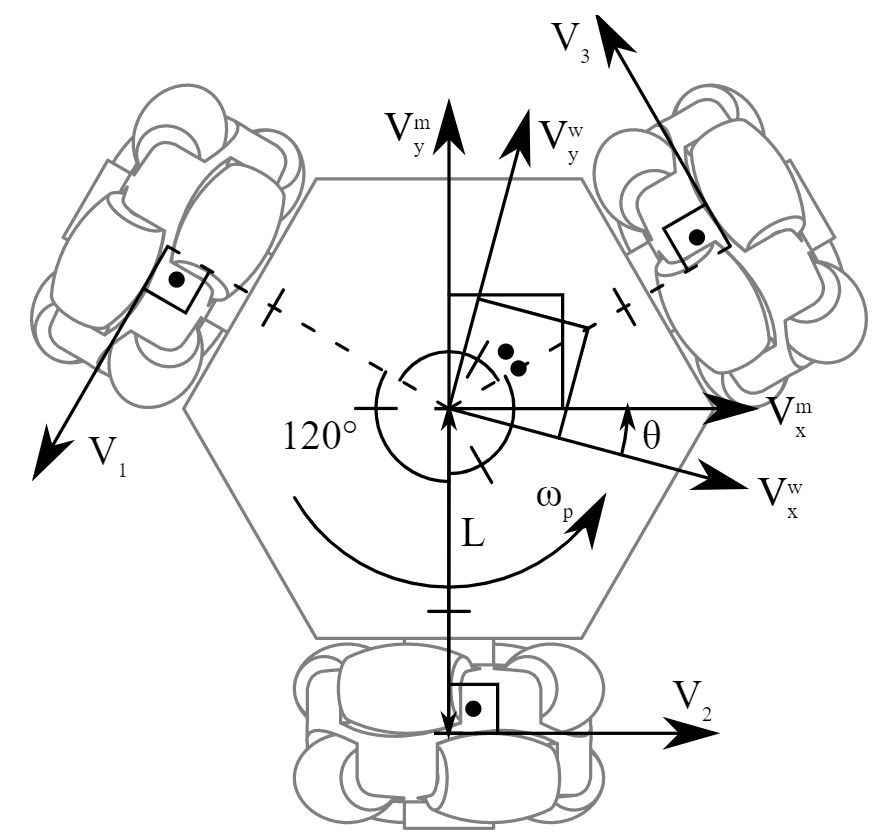
\includegraphics[width=100mm]{graphics/omnischeme.png}
  \caption{Schemat ukazujący poszczególne wektory prędkości}
  \label{fig:forklift}
\end{figure}

Równania kinematyczne odnoszące się do punktu odniesienia robota:
\begin{gather*}
 V_x^m = \frac{2 \cdot V_2 - V_1 - V_3}{3} \\
 V_y^m = \frac{\sqrt{3} \cdot V_3 - \sqrt{3} \cdot V_1}{3} \\
 \omega_p = \frac{V_1 + V_2 + V_3}{3 \cdot L}
\end{gather*}

Równania kinematyczne odnoszące się do punktu odniesienia świata:
\begin{gather*}
 V_x^w = \cos{\theta} \cdot V_x^m - \sin{\theta} \cdot V_y^m\\
 V_y^w = \sin{\theta} \cdot V_x^m + \cos{\theta} \cdot V_y^m\\
\end{gather*}

Kinematyka odwrotna w układzie odniesienia robota:
\begin{gather*}
 V_x^m = \cos{\theta} \cdot V_x^m + \sin{\theta} \cdot V_y^m\\
 V_y^m = -\sin{\theta} \cdot V_x^m + \cos{\theta} \cdot V_y^m\\
\end{gather*}

Kinematyka odwrotna w układzie odniesienia świata:
\begin{gather*}
 V_1 = - \frac{V_x^m}{2} - \frac{\sqrt{3} \cdot V_y^m}{2} + L \cdot \omega_p \\
 V_2 = V_x^m + L \cdot \omega_p \\
 V_3 = - \frac{V_x^m}{2} + \frac{\sqrt{3} \cdot V_y^m}{2} + L \cdot \omega_p
\end{gather*}

Za pomocą powyższych wzorów modelu kinematycznego pojazdu, zrealizowano
odometrię oraz sterowaniem robotem.


\section{System wizyjny}
\subsection{Sprzęt wizyjny}
Jako bazę do wyznaczania ścieżki robota w~terenie zdecydowano się użyć kamery
\textit{Raspberry Pi Camera V2}, która oferuje obraz wideo w~rozdzielczości
\textit{full HD} oraz zdjęcia w~rozdzielczości do \textit{4K}.
Kamera jest wyposażona we wbudowany obiektyw szerokokątny, co jest korzystne
w~zastosowaniach robotyki.

\subsection{Wyznaczanie przestrzeni ruchów robota}
Kamerę przygotowano do wykorzystania w~celu wykonywania zdjęcia labiryntu,
w~którym poruszać może się robot.
Obraz z~kamery należy przetworzyć aby uzyskać mapę przestrzeni, po której może
poruszać się robot.
Biała przestrzeń na mapie powinna oznaczać miejsca, w których może znaleźć się 
środek robota, czarne pola to miejsca zabronione (przeszkody oraz ich
margines).
Budowę mapy wykonano w~następujących krokach:
\begin{itemize}
	\item binaryzacja zdjęcia z kamery,
	\item wykrycie położenia robota oraz jego promienia na podstawie markerów,
	\item usunięcie obrysu robota z~przestrzeni zabronionej, 
	\item naniesienie marginesu przeszkód.
\end{itemize}

Ze względu na zdalny charakter pracy w~semestrze letnim 2020 przygotowano
prototypowy model labiryntu.
Podstawą przetwarzania obrazu labiryntu jest binaryzacja metodą
\textit{isodata}.
Oparcie wizji na algorytmie binaryzacji wymaga odpowiedniego kontrastu zdjęcia
oraz dobrego oświetlenia labiryntu.
\textit{Isodata} jest adaptacyjną metodą binaryzacji zdjęć, która gwarantuje,
że wartość progowania jest średnią ze średnich wartości ekspozycji podzielonych
fragmentów zdjęcia.
Taki algorytm binaryzacji odpowiada algorytmowi klasteryzacji
\textit{k-średnich}, gdzie \textit{k} wynosi dwa.
Przykładowy labirynt po binaryzacji przedstawiono na rysunku
\ref{fig:maze_bin}.
\begin{figure}
\centering
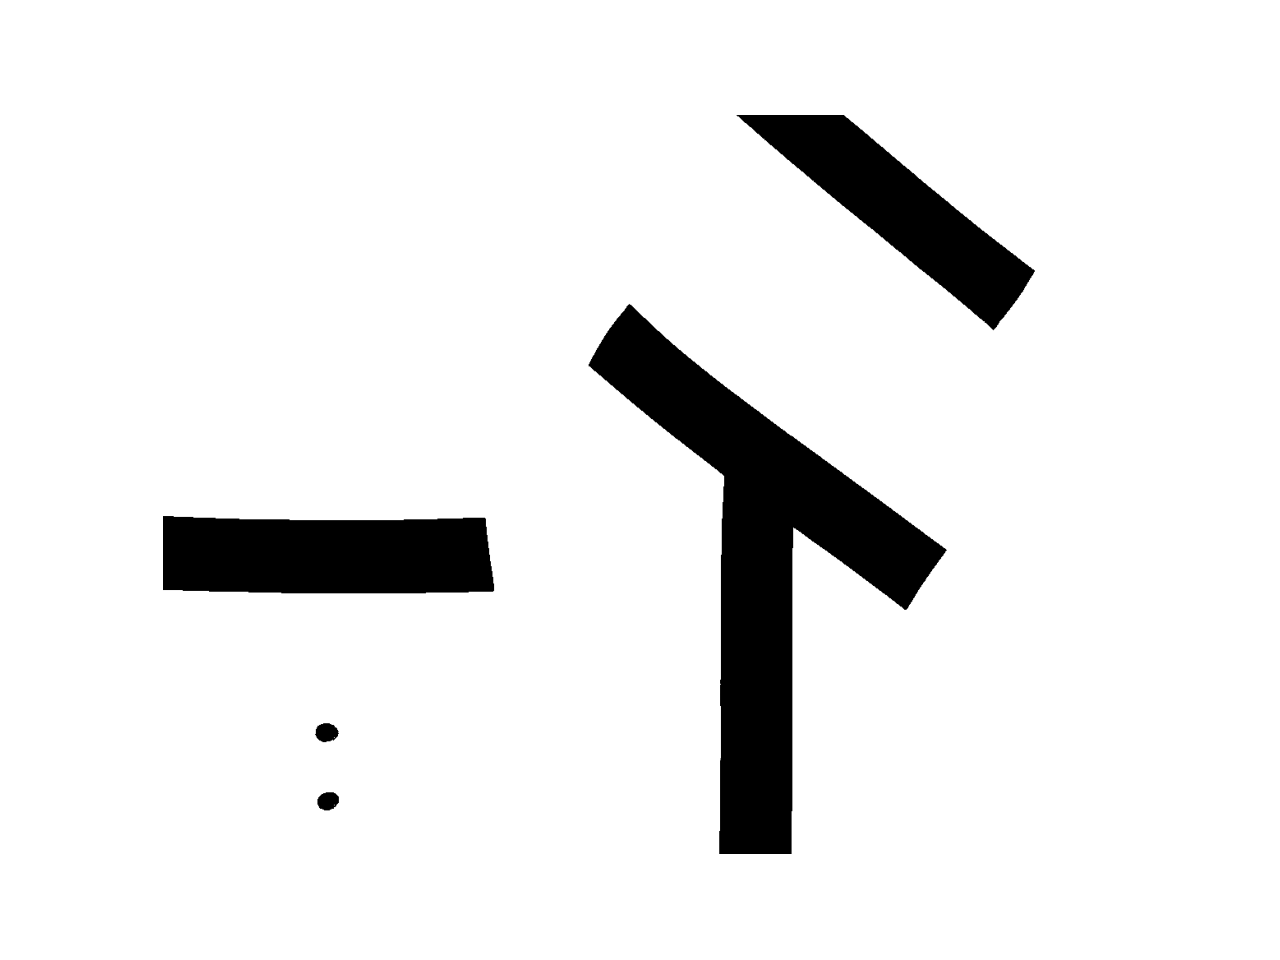
\includegraphics[width=0.5\textwidth]{maze_bin.png}
\caption{Przykładowy labirynt poddany binaryzacji}
\label{fig:maze_bin}
\end{figure}

W~następnym kroku algorytm wizyjny przeprowadza wykrycie pozycji i~rozmiaru
robota na podstawie dwóch czerwonych markerów umieszczonych na jego obwodzie.
Punkty o charakterystycznym kolorze najlepiej wykrywać w~przestrzeni barw HSV
(barwa, nasycenie, jasność ang. \textit{hue, saturation, value}).
W~omawianej przestrzeni kolory są reprezentowane przez wartość kąta; od zera do
kąta pełnego, przy czym wartości reprezentuje często się jako ułamek dziesiętny
z~maksymalnej wartości.
Kolor czerwony jest w~takim systemie opisywany przez kąty zbliżone do zera.
Markery zdecydowano się kwalifikować w~przedziale odcieni czerwonego od 0,9 do
1~oraz 0~do 0,1.
Wartości nasycenia oraz jasności markerów są akceptowane dla wartości większych
od 0,3.
Po progowaniu pozycji markerów dokończono proces ich segmentacji przez
etykietowanie oraz obliczenie parametrów obszaru zajmowanego przez markery.
Wyznaczono ich centroidy; punkt między centroidami markerów to środek robota.
Po wyznaczeniu pozycji robota można usunąć jego kształt z~mapy przez odjęcie
maski jego obrysu z obrazu.
Wyniki omówionych operacji przedstawiono na rysunkach \ref{fig:maze_markers}
oraz \ref{fig:maze_rm_markers}.
\begin{figure}
\centering
\hfill
\begin{subfigure}[b]{0.45\textwidth}
	\centering
	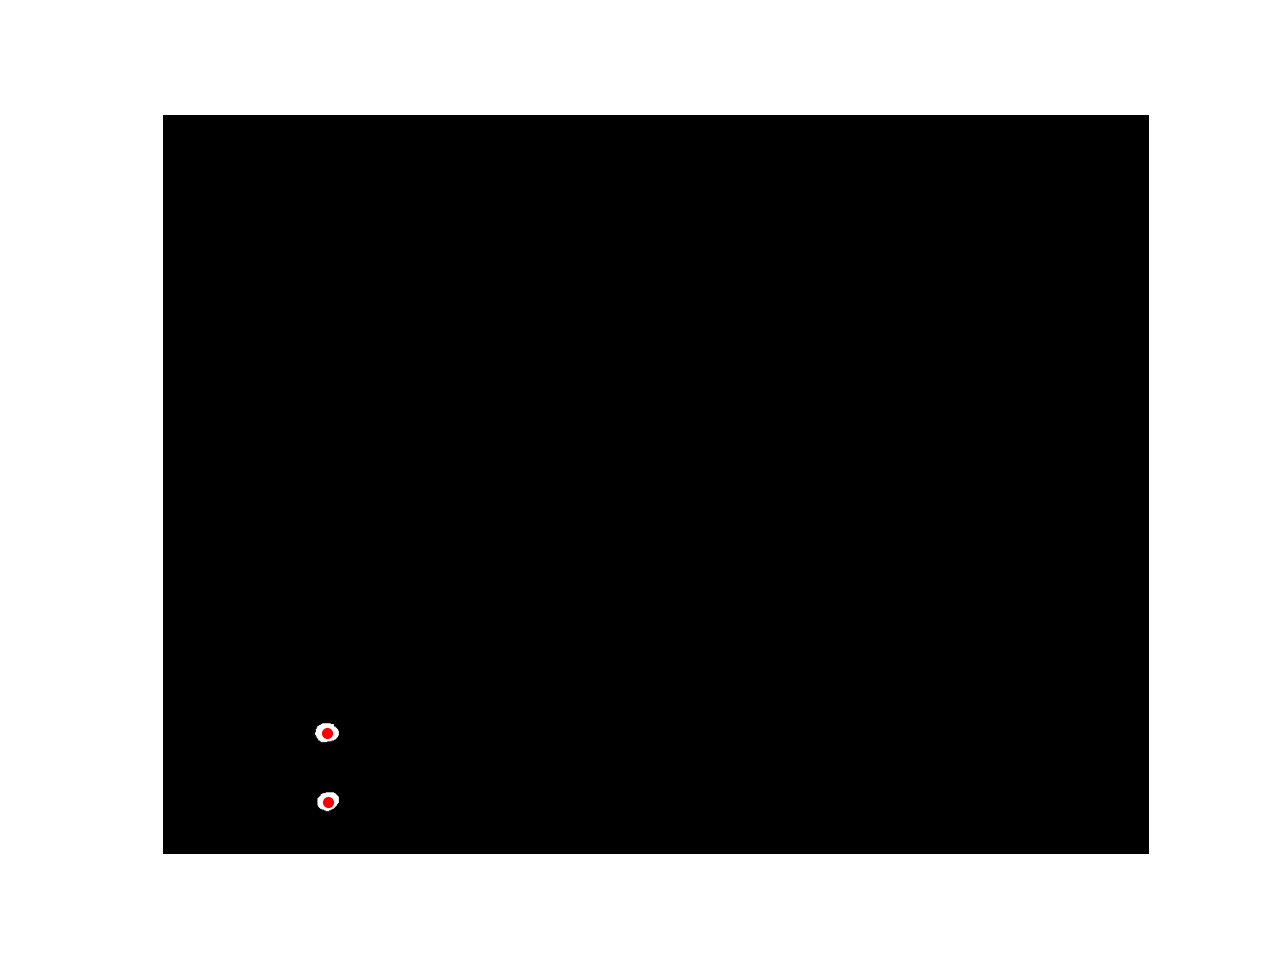
\includegraphics[width=\textwidth]{maze_markers.png}
	\caption{Wykryte markery i~ich centroidy}
	\label{fig:maze_markers}
\end{subfigure}
\hfill
\begin{subfigure}[b]{0.45\textwidth}
	\centering
	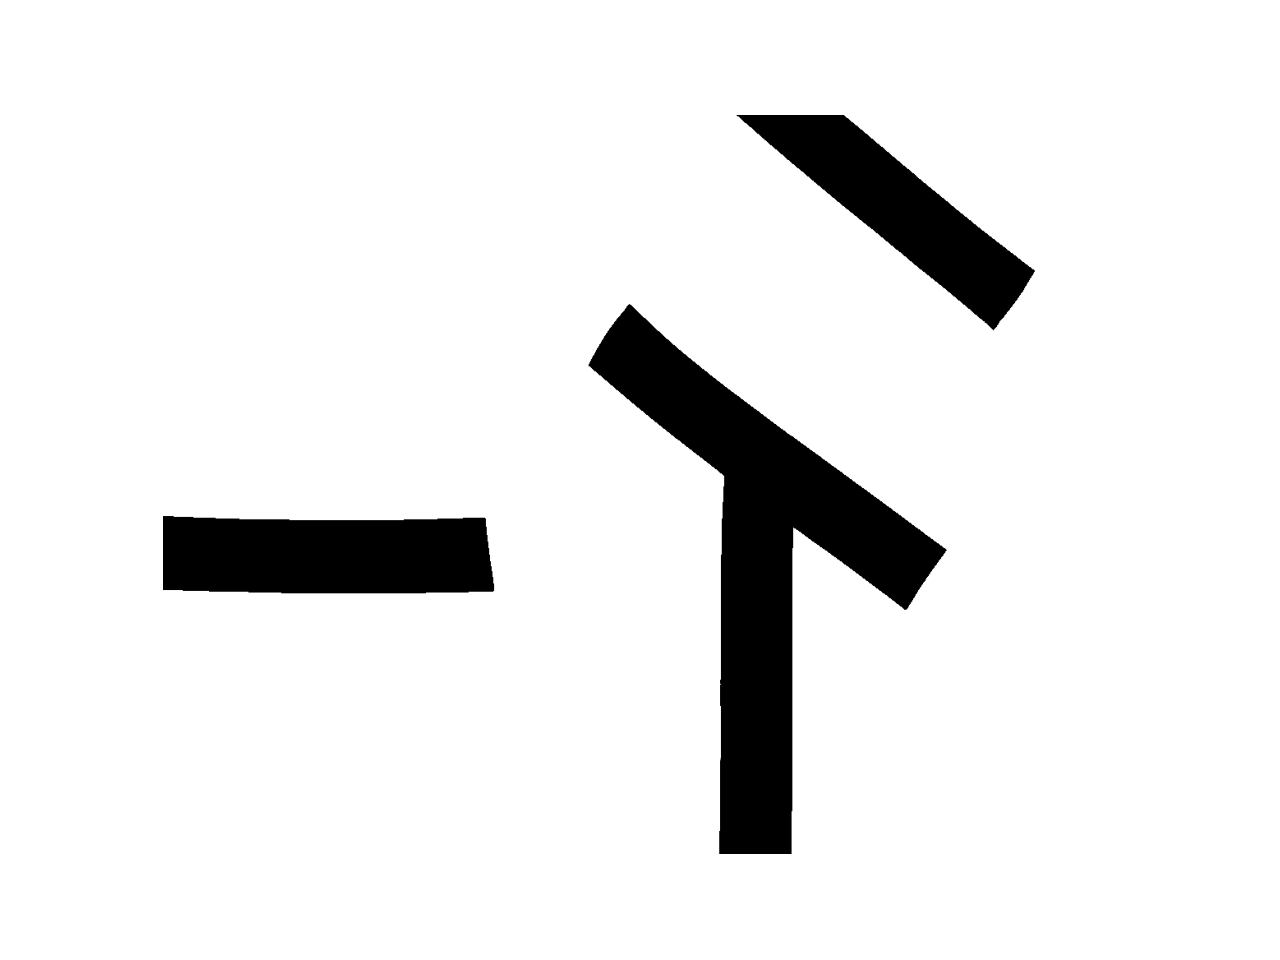
\includegraphics[width=\textwidth]{maze_rm_markers.png}	
	\caption{Labirynt po usunięciu markerów}
	\label{fig:maze_rm_markers}
\end{subfigure}
\hfill
\caption{Wykrywanie oraz usuwanie markerów z~mapy labiryntu}
\end{figure}

Ostatni etap przygotowania mapy polega na dodaniu do ścian labiryntu marginesu,
który zapewni, że krawędź robota nie zetknie się z przeszkodami.
W~tym celu dokonano procesu erozji binarnej przestrzeni dozwolonej ruchu
robota.
Margines ścian wyznaczono na podstawie średnicy robota wyznaczonej przy
segmentacji markerów.
Erozji dokonano używając jądra w~kształcie okręgu o~promieniu równym ponad
połowie promienia robota.
Ostatecznie powstaje mapa binarna, na której kolor biały oznacza przestrzeń
w~której może znaleźć się środek robota, przedstawiono ją na rysunku
\ref{fig:maze_walls}
\begin{figure}
\centering

\includegraphics[width=0.5\textwidth]{maze_walls}
\caption{Przykładowy labirynt z~naniesionym marginesem ścian}
\label{fig:maze_walls}
\end{figure}

Do wykonania wymienionych operacji użyto funkcji z~biblioteki
\textit{scikit-image} dla języka Python.

\section{Analiza biznesowa}
W~ramach projektu dokonano analizy możliwości biznesowych związanych z~robotyką
mobilną w~regionie Górnego Śląska.
Pełną treść analizy zamieszczono w~osobnym dokumencie.

\subsubsection{Przegląd dostępnych źródeł finansowania}
Przeanalizowano ofertę dofinansowania projektów oraz przedsięwzięć biznesowych:
zarówno krajowych, jak i zagranicznych.
W~ramach przeglądu wzięto pod uwagę oferty aktualne oraz niedawno zakończone.
Dofinansowania w~ramach programów rozwoju oraz inkubatorów charakteryzowały się
atrakcyjnymi ofertami, niektóre z~nich nie wymagały wkładu własnego, inne
uzależniały go od wysokości kwoty pomocy.
Wkład własny większości rozpatrywanych programów nie przekraczał parunastu
procent.
Oferty proponowały wsparcie w~wysokości od parudziesięciu do paruset tysięcy
złotych.
Częstym wymogiem uczestnictwa w~programie była gotowości prototypu produktu.
Wsparcie w~projektach jest ograniczone do małych firm, przy czym pożądana jest
współpraca z~uczelnią.
W~ramach przeglądu analizowano programy takie jak: \textit{POWER},
\textit{Program Akceleracyjny KPT} oraz \textit{Program Inteligentny Rozwój}.

\subsubsection{Przykłady rozwijających się firm na rynku robotyki}
Spośród polskich działalności przeanalizowano rozwój firm takich jak
\textit{KP Labs} oraz \textit{Future Processing}.
Zwrócono uwagę na źródła finansowania projektów.
Produkty o~wysokiej innowacyjności i~aspekcie naukowym (takie jak w~przypadku
firmy \textit{KP Labs}) uzyskały bardzo wysokie dofinansowania unijne,
przekraczające połowę wartości poszczególnych przedsięwzięć.
Produkty związane na przykład z~kosmonautyką mogły liczyć na dotacje wielkości
milionów złotych.

Zdecydowano się także na analizę zagranicznych firm, które w~ostatnich latach
odniosły sukces na arenie międzynarodowej.
Zwrócono uwagę na działalność skandynawskiej firmy \textit{Antmicro}, która
posiada polskie filie.
Wiele z~wykorzystywanych przez firmę technologii należy do grupy \textit{open
source} oraz \textit{open source hardware}.
Ciekawym przypadkiem okazała się inicjatywa \textit{CommaAI}, której twórcą
jest znany programista Georg Hotz.
Jego firma skupia się na wyposażaniu istniejących samochodów, w~systemy jazdy
autonomicznej.
\textit{CommaAI} oferuje oprogramowanie oraz moduły współpracujące z~czujnikami
i~kamerami wbudowanymi w~samochody oraz smartfony.
Jest to ciekawe podejście wykorzystujące wykosi poziom cyfryzacji otaczających
technologii.
Takie podejście ułatwia tworzenie produktów oraz pozwala na oferowanie ich
w~konkurencyjnych cenach.

\subsubsection{Analiza SWOT potencjalnego przedsięwzięcia}
W~ramach analizy przeprowadzono analizę \textit{SWOT} hipotetycznego
przedsięwzięcia w~dziedzinie robotyki mobilnej w~warunkach biznesowych Górnego
Śląska.
Analiza skupia się na możliwościach założenia działalności biznesowej przez
absolwentów Politechniki Śląskiej.

\paragraph{Mocne strony}
\begin{itemize}
	\item potencjalni członkowie zespołu, tzn. absolwenci kierunków technicznych
		  są zapoznani z~bieżącymi, nowoczesnymi technologiami,
	\item potencjalni członkowie zespołu rozumieją potrzeby nowoczesnego
		  przemysłu.
	\item dobry wewnętrzny kontakt absolwentów z uczelnią.
\end{itemize}

\paragraph{Słabe strony}
\begin{itemize}
	\item potencjalni członkowie zespołu (absolwenci, doktoranci) mają małe
          doświadczenie biznesowe i~menadżerskie.
\end{itemize}

\paragraph{Szanse}
\begin{itemize}
	\item zainteresowanie medialne i społeczne nowymi technologiami,
	\item liczne projekty dofinansowania; unijne oraz krajowe,
    \item możliwość współpracy z jednostkami naukowymi i uczelniami badawczymi.
\end{itemize}

\paragraph{Zagrożenia}
\begin{itemize}
	\item nieprzygotowanie polskiego rynku na adaptowanie nowych technologii,
	\item prawdopodobny kryzys,
	\item ryzyko przejęcia firmy przez zagraniczny koncern, ze względu na brak
          bezpośredniego odbiorcy zaawansowanych produktów na rodzimym rynku.
\end{itemize}

\section{Podsumowanie}
W ramach projektu zaprojektowano model 3D robota mobilnego, a następnie
stworzono symulację, która pozwala na implementację oraz testowanie
poszczególnych algorytmów.

Wykorzystując platformę ROS stworzono architekturę węzłów, która pozwoli na
łatwą integrację z rzeczywistym obiektem, co może być podstawą do kontynuowania
projektu.

Za pomocą wyznaczonego modelu kinematycznego pojazdu stworzono węzeł, który
określa odometrie pojazdu, na podstawie symulowanych danych z enkodera.

Opracowano system AHRS bazujący na filtrze Kalmana.
System wyznaczania orientacji w~przestrzeni zaimplementowano i~przetestowano
z~użyciem systemu mikroprocesorowego.

Wykonano prototyp systemu wizyjnego wyznaczającego przestrzeń dozwoloną robota
w~labiryncie.

W~raporcie załączono wnioski wynikające z~przeprowadzonej analizy rynku
pojazdów autonomicznych oraz analizę ryzyka przedsięwzięcia tego typu.


% Lists of objects
\listoffigures
\listoftables
\listoflistings

% Bibliography
\nocite{*}
\bibliographystyle{plplain}
\bibliography{references}

\end{document}
